\chapter{Related Work}
\label{ch:related-work}

% You will need to describe what has been done before and you will need to discuss the theory that your work is based upon. This is a slightly dangerous: Take care not to punish the reader with hairy theory without explaining why it is needed.

% What is the main idea? What is the contribution (the new or interesting thing)? What is important for you? Where it is presented?

% Gist + My comment
% TODO: go through each paper and make short notes on what's important and why.

The method presented in this paper builds upon the previous work on wrapper induction, HTML aware data extraction, probabilistic tree-edit distance measures, and data record mining. The most influential ideas are covered in this chapter.


% ---------------------------------------------------------------------
\section{Wrapper Induction Method Overview}
% discuss classification and state our focus

The problem of data extraction, especially from web pages, has been addressed in a number of papers. Laender et al. \cite{Laender:2002:BSW:565117.565137} group wrapping techniques into multiple categories, including natural language processing, languages and grammar, machine learning, information retrieval, databases, and ontologies. A common goal of all wrapper generation tools is to build a wrapper that is both accurate and robust, but is built with the least possible human interaction. The article provides a taxonomy for grouping wrapping techniques.

The most relevant category mentioned in the paper is the HTML-aware tools. These rely on structural features of HTML documents. The document is parsed into a tree structure and extraction rules are applied to the tree. Although the tools discussed (XWRAP, W4F, RoadRunner) provide a high degree of automation, many of them rely on heuristics and have a weak notion of robustness.

In a more recent overview of web data extraction techniques \cite{Chang:2006:SWI:1159162.1159300}, Chang et al. argue, that due to template generated content, web information extraction can take advantage of machine learning and pattern matching methods, while traditional approaches are mostly based on natural language processing. The author argues, that unsupervised approaches can only support pages based on a template. The extension of such extraction tasks to support non-template based pages is very limited.

Our research deals with data extraction from HTML documents, which are semi-structured by definition. Thus, we focus on the techniques based on structural features rather than vague natural language processing, which requires large training sets. Yet, the content features are also interesting for extra accuracy, but we leave it for future work.

% wrapper induction system
\begin{figure}[h]
	\centering
	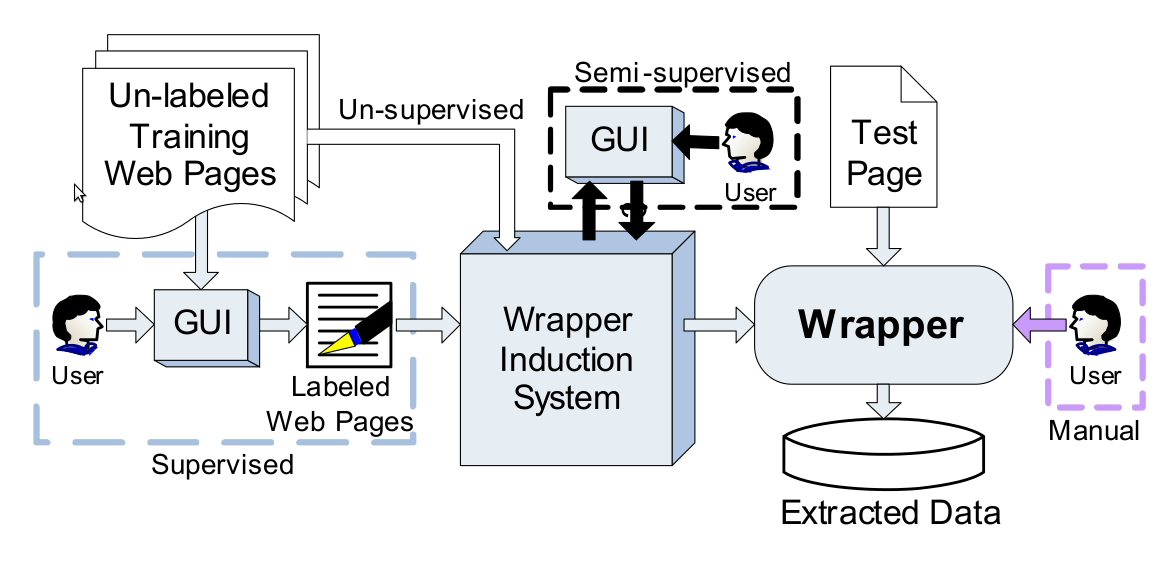
\includegraphics[width=1.0\textwidth]{figures/wrapper-induction}
	\caption{Wrapper induction system as described by Chang et al. \cite{Chang:2006:SWI:1159162.1159300}.}
	\label{fig:wrapper-induction}
\end{figure}

Zhai and Liu \cite{zhai2005a} report, that there are two main methods for data record extraction: wrapper induction and automatic extraction. In wrapper induction (see Figure~\ref{fig:wrapper-induction}), a user manually annotates a set of pages and extraction rules are learnt. Data extraction from future pages are based on these rules. The problem with this method is that it requires a fairly large set of manually labeled pages. In automatic extraction, patterns are identified from multiple pages. A major limitation is that pages have to be clustered by similarity, which is again a manual process.


% ---------------------------------------------------------------------
\section{HTML Aware Data Extraction}
% elaborate on the research in the area of our focus

% IBM Report: Robust Web Data Extraction with XML Path Expressions
One the the first papers to discuss XPath based wrappers was \cite{Myllymaki02robustweb}. In this work, XML tools are used convert HTML document into pure XHTML and later XPath queries extract desired pieces of information. The wrapper is a set of XSLT extraction rules, i.e. hops that are based on structure, attributes, or content. Yet, the actual XPath queries were written by hand without much automation.

The same paper mentions \emph{robustness} as a feature of a good extraction rule. The author informally defines robustness as the ability to extract intended data from an HTML page after structural changes to the page. Two metrics for measuring robustness are introduced. The first is a number of times that expression failed to extract correct results. The second is expression complexity in terms of depth. The paper defines a notion of \emph{anchors} (DOM tree nodes) and \emph{hops} (relative XPath expressions) over a normalized HTML document. 

% Relative vs absolute queries: Robust Web Content Extraction
Chang et al. \cite{Chang:2006:SWI:1159162.1159300} mention techniques that improve the robustness of XPath expressions. A general approach of these methods is to rewrite the query in a way that it depends on more stable elements of HTML tree. This is achieved by tracking structural changes in the training set. \cite{Kowalkiewicz:2006:RWC:1135777.1135928} empirically confirmed that there is a notable difference between various versions of wrappers in terms of robustness -- a relative XPath expressions outperform absolute ones significantly. This proves the idea that some wrappers are more robust.

% Vertex tool
Gulhane et al. \cite{DBLP:conf/icde/GulhaneMMRRSSTT11} introduce apriori style algorithm for learning XPath-based extraction rules that are robust to variations in site structure. Algorithm learns structural rules from human annotated pages. Based on domain knowledge, these features are classified into strong (e.g. HTML attributes \texttt{class} or \texttt{id}, tags, textual fragments) and weak (e.g. \texttt{font}, \texttt{width} attributes). This method tries to build an XPath query from strong features only by generating and combining candidates. If apriori fails to output precise XPath, Naive-Bayes based classifier is used to evaluate the best guess of newly generated nodes with weak features. Essentially, this method is based on enumeration, which makes it slow for large websites. Additional limitations are the use of large training set and that it requires a set of annotated pages for certain heuristics (e.g. support metrics) to properly work. 

% WebSelF tool
Thomsen et al. \cite{Thomsen:2012:WWS:2364120.2364156} present a framework that takes into account not only the structure and the content of a scrapped page, but also the context and the presentation, i.e. the location where the data is physically located after full rendering and applying stylesheets. It also works with dynamic page elements, that are frequent in JavaScript rich web pages. The design of the framework consists of three type of functions: for selecting elements, for for verifying the selected elements, and for maintaining the previous functions. Complementing structural information with visual details is an interesting direction, but we focus on just the structure.


% ---------------------------------------------------------------------
\section{Tree-Edit Distance}
\label{sec:tree-edit-distance}

% A Survey on Tree Edit Distance and Related Problems
In a recent survey on tree-edit distance problem by Bille \cite{bille2005a} a number of solutions are overviewed. While it has been shown that edit distance problem is NP-complete for unordered trees, for ordered trees dynamic programming algorithms exist. Several algorithms have been proposed, among them Shaha and Zhang \cite{shasha1990a} and Demaine et al. \cite{demaine2007a} with time complexity of $O(m^2 n^2)$ and $O(n^ 2m(1+\log_m n))$  for trees with $m$ and $n$ nodes respectively. The efficiency of the two algorithms heavily depends on the tree shape and it is hard to chose between them. 

% RTED - A Robust Algorithm for the Tree Edit Distance
Addressing this problem, a robust algorithm \emph{RTED} has been proposed by Pawlik and Augsten \cite{pawlik2011a}. \emph{RTED} is not only tree-shape independent, but for any problem instance computes as many relevant subproblems as the best competitor must compute. \emph{RTED} runs in $O(n^3)$ time and in many cases outperforms the competitors. Moreover, the authors provide a Java library for use in own projects. Thus, we use \emph{RTED} in our data record mining algorithm.

% Automatic web news extraction using tree edit distance by Reis'04
Alternatively, a number of restricted tree-edit distance algorithms exists. For example, in \cite{de2004a} Reis et al. introduce a \emph{Restricted Top-Down Mapping} algorithm, which calculates edit-tree distance by efficiently analysing tree structure. Generally, the algorithm imposes top-down mappings which allow removal and inserts at the bottom of the tree only. It is based on assumption that just the content at the bottom of the elements changes. We discard these algorithm variations as too focused on edge cases and not suitable for a general use-case.


%----------------------------------------------
\section{Probabilistic Change Model}

% [Dalvi'09] Probabilistic change model
Essential ingredient in tree-edit distance calculations is the actual cost of each edit operation. However, none of the algorithms discussed define the \emph{probability distribution}, i.e. they assume that the costs are provided. Clearly, assumption that each transformation has a unit cost does not represent the real world. Dalvi et al. \cite{dalvi2009a} show that certain operations are more probable than others. Authors use iterative numerical methods to estimate the \emph{change model}, i.e. probability distribution, from a set of web page snapshots.

Having probabilities of edit operations and a method for calculating tree-edit distance, we can now efficiently compute the probability of one tree evolving into the other. This allows to formally define wrapper \emph{robustness} as the ability for the wrapper to work on the future snapshots of the web page. 

% [Dalvi'09] Robust Web Extraction - An Approach Based on a Probabilistic Tree-Edit Model
Extending this idea, Dalvi et al. \cite{dalvi2009a} build a robust web extraction framework (see Figure~\ref{fig:web-extraction-framework}).  The method generates a set of candidate XPath wrappers and selects the most robust one. The problem with this approach is that it picks the local optimum from a generated set, rather the provably global optimum.

% Robust web extraction framework
\begin{figure}[h]
	\centering
	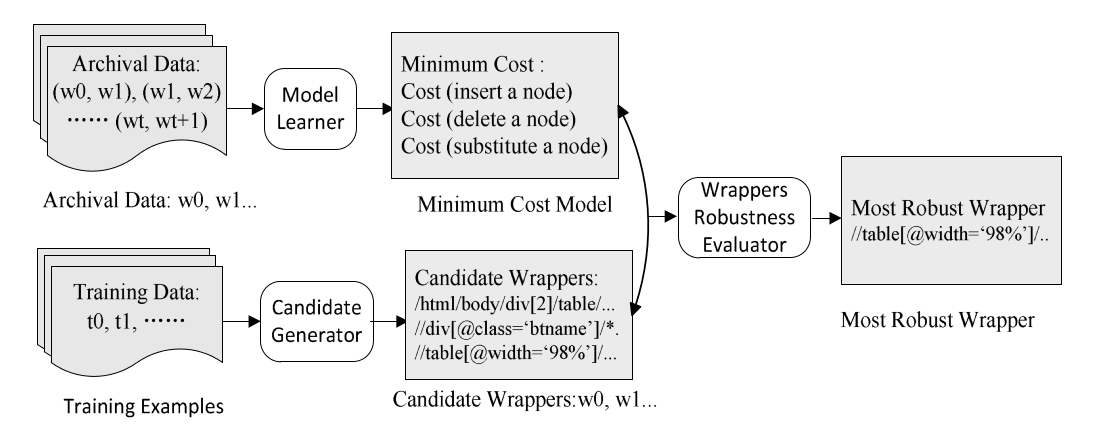
\includegraphics[width=\linewidth]{figures/robust-web-extraction-framework}
	\caption{Robust web extraction framework.}
	\label{fig:web-extraction-framework}
\end{figure}

% [Parameswaran'11] Optimal Schemes for Robust Web Extraction
Parameswaran et al. \cite{DBLP:journals/pvldb/ParameswaranDGR11} elaborate the concept of robustness and provide a method for building wrappers with provably optimal robustness. Two robustness models are introduced: the worst case and the most probable case. An algorithm for computing optimal wrapper in polynomial running time is introduced. Yet, it relies on enumeration to compute the minimum cost scripts and to extract the distinguished node \cite{DBLP:conf/wism/LiuWYL12}.

% Discussion
We could not find alternative formal definitions of wrapper robustness that took into account structural properties of HTML documents. Combined with a number of heuristics (alignments, subforest optimization, early pruning, etc.), robust web extraction proves to be both accurate and fast. Both of the features that are required in our wrapper. The only major problem with approach, is that it only supports single distinguished node per HTML document. Thus, we need a good way to separate individual data records.


% ---------------------------------------------------------------------
\section{Data Record Mining}

% Data record mining
Liu et al. \cite{liu2009a} propose a \emph{Mining Data Records} (MDR) algorithm for automatically locating data records in web pages. In other words, MDR finds page regions generated by a template. The method is based on (1) string edit distance algorithm to find data records and (2) two observations about data records in an HTML document. First, a group of data records have similar tree structure and are located in a close proximity. Second, these groups are under one parent node, i.e. it is very unlikely that a single record would begin inside one child subtree and end inside another child subtree. The algorithm works both with continuous and noncontinuous data regions. 

% discussion
We find this method to be efficient, as it does not require training set and is fast. However, we believe that tree-edit distance is more accurate measure than string matching in HTML documents.

% Web data extraction based on partial tree alignment
Building on Liu et al. work \cite{liu2009a}, Zhai and Liu further develops the idea of extracting data from a web page that contains several structured data records \cite{zhai2005a}. Their method is based on visual clues: style and position of elements after rendering. After identifying individual data records, the proposed approach aligns multiple tag trees into a generic \emph{seed tree}. The seed tree contains a maximum number of data record fields.

% Joint Optimization of Wrapper Generation and Template Detection
% Efficient record-level wrapper induction
Similarly, in \cite{zheng2007a} the DOM tree is progressively converted into a generic page-level wrapper tree. A cost-driven dynamic programming is employed for the alignment algorithm. The issue with this approach is that tree-mapping operations are expensive. Zheng et al. further develop tree alignment idea \cite{DBLP:conf/cikm/ZhengSWG09} and introduce a concept of \emph{broom} structure, which effectively is a generalized tree for record wrapping by alignment. Basically, the template is reconstructed from multiple HTML fragments. By restricting alignment to relevant DOM regions, the tree alignment cost is reduced dramatically. It also handles case of cross records and uses content matching for improved record extraction.

% discussion
Both of the aforementioned tree alignment techniques present an interesting idea in record-level wrapping. They both try to reconstruct the template by generalizing multiple records into a generic template tree. We further explore this idea in our wrapper design.


% vim:wrap linebreak nolist:
